\section{双平方根方程的意义}
\label{sec:3.4}

双平方根方程具有石油勘探地震数据处理中大多数非统计方法方面的特点.这种在前一
节中导出的方程颇不易于理解,因为它是一种在四维空间$(z,s,g,t)$中的算子。我们将
通过各种具体应用来对它进行探讨,在各该应用中它均是一种较低维空间中的问题。在本节
中,速度横向变化将忽略不计(因为事情本来就够复杂的了,要考虑它就更棘手了)。讨论
就从下列二式开始:

\begin{subequations}
\begin{equation}
\frac{dU}{dz}=-\frac{i\omega}{v}[\sqrt{1-G^2}+\sqrt{1-S^2}]U
\label{eq:ex3.4.1a}
\end{equation}
\begin{equation}
\frac{dU}{dz}=-\frac{i\omega}{v}[\sqrt{1-(Y+H)^2}+\sqrt{1-(Y-H)^2}]U
\label{eq:ex3.4.1b}
\end{equation}
\label{eq:ex3.4.1}
\end{subequations}

\subsection{零炮检距偏移$(H=0)$}
\label{sec:3.4.1}

降低\ref{eq:ex3.4.1b}之维数的一种办法就是直接令$H=0$,于是两个平方根变得相同,从而
可将它们合并,得出熟悉的旁轴方程

\begin{equation}
\frac{dU}{dz}=i\omega\frac{2}{v}\sqrt{1-\frac{v^2k_y^2}{4\omega^2}}
\label{eq:ex3.4.2}
\end{equation}

在式\ref{eq:ex3.4.2}中出现岩石速度的两个地方,该岩石速度均应除以2,这是由于为使野外资料
与爆炸反射面模型相应,就需要使岩石速度减半。所以不论我们作过了什么,只要是令$H=0$,
我们就得到在第一章中使用过的方程了。令$H=0$就使观测排列延拓概念在作用上有等价于
爆炸反射面概念的效果了。

\subsection{零倾角叠加$(Y=0)$}
\label{sec:3.4.2}

处理炮检距$h$的时候,通常假设地层是水平成层的,从而观测结果将与中心点$y$无关。除
了或换句话说,除以外,采用这样一种地层模型时,所有遍及$y$之数据资料的
Fourier变换均将为零。当$Y=0$时,式\ref{eq:ex3.4.1}中的两个平方根又变得相等,因而所得方
程再一次成为旁轴方程

\begin{equation}
\frac{dU}{dz}=i\omega\frac{2}{v}\sqrt{1-\frac{v^2k_h^2}{4\omega^2}}
\label{eq:ex3.4.3}
\end{equation}

利用这个方程将双曲面从地表向下延拓时,可发现双曲面随着深度之增大而蜷缩,直至达到
出现最佳聚焦的正确深度,这种情形如图\ref{fig:ofs/dc2}所示。

各波均在零炮检距时出现最佳聚焦。出现聚焦代表向下延拓达到目的,这时,向下延拓
正好到达一个反射面。对于正位于反射面之上的自激自收点的情形,是在零值旅行时间上的
反射最强。采集$t=0$时在零炮检距上的值并放弃其余炮检距上的值,是消除干扰的一种途径
(实际上,这就是一种限制干扰影响的方法)。粗略地说,这同沿着原始资料上的双曲线轨
跡进行求和的常规处理过程就是一回事。很自然,向下延拓处理时采用的波速最接近于地层
速度时,求和可望达到最隹状态。以后就将利用炮检距空间来测定速度。


\subsection{常规处理---近似分离法}
\label{sec:3.4.3}

将式\ref{eq:ex3.4.1b}括号中的算子在形式上定义为双平方根算子(DSR算子)
\begin{equation}
\text{DSR}(Y,H)=\sqrt{1-(Y+H)^2}+\sqrt{1-(Y-H)^2}
\label{eq:ex3.4.4}
\end{equation}

\begin{figure}[H]
\centering
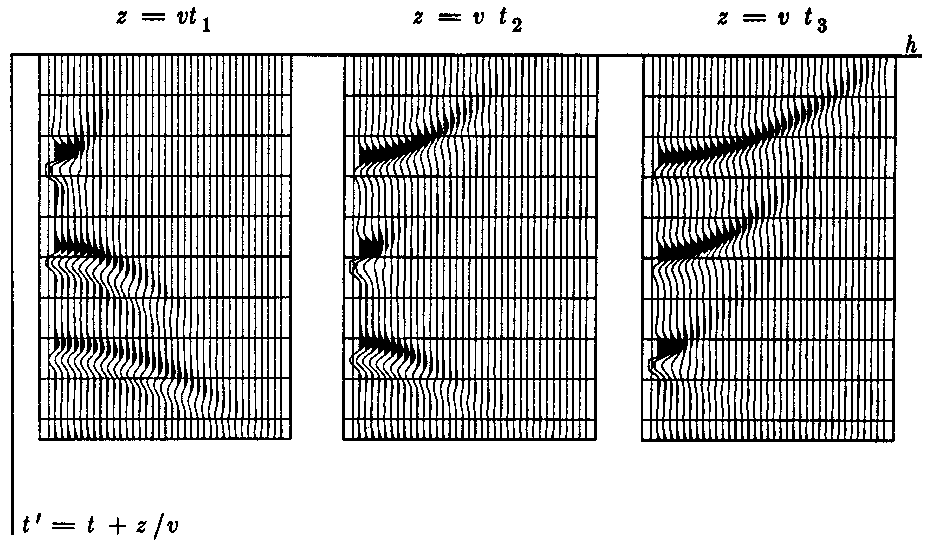
\includegraphics[width=0.65\textwidth]{ofs/dc2}
\caption[chervon]{采用三层的地层模型时,共中心点道集为三个双曲面。连续图形表示
向下延拓相继达到出现最佳聚焦时的深度}
\label{fig:ofs/dc2}
\end{figure}

在Fourie空间内,向下延拓是用相移因子$exp(i\omega \text{DSR}\frac{z}{v})$完成的。
